\chapter{Introduction à ShankScript}


\section{Qu'est ce que ShankScript ?}


En informatique, un langage de programmation est une notation conventionnelle destinée à formuler des algorithmes et produire des programmes informatiques qui les appliquent. D'une manière similaire à une langue naturelle, un langage de programmation est composé d'un alphabet, d'un vocabulaire, de règles de grammaire et de significations .
\\[0.5cm]
Les langages de programmation permettent de décrire d'une part les structures des données qui seront manipulées par l'appareil informatique, et d'autre part d'indiquer comment sont effectuées les manipulations, selon quels algorithmes. Ils servent de moyens de communication par lesquels le programmeur communique avec l'ordinateur, mais aussi avec d'autres programmeurs ; les programmes étant d'ordinaire écrits, lus, compris et modifiés par une équipe de programmeurs .
\\[0.5cm]
Un langage de programmation est mis en œuvre par un traducteur automatique : compilateur ou interpréteur. Un compilateur est un programme informatique qui transforme dans un premier temps un code source écrit dans un langage de programmation donné en un code cible qui pourra être directement exécuté par un ordinateur, à savoir un programme en langage machine ou en code intermédiaire, tandis que l'interpréteur réalise cette traduction « à la volée ».
\\[0.5cm]
Les langages de programmation offrent différentes possibilités d'abstraction, et une notation proche de l'algèbre, permettant de décrire de manière concise et facile à saisir les opérations de manipulation de données et l'évolution du déroulement du programme en fonction des situations. La possibilité d'écriture abstraite libère l'esprit du programmeur d'un travail superflu, notamment de prise en compte des spécificités du matériel informatique, et lui permet ainsi de se concentrer sur des problèmes plus avancés.
\\[0.5cm]
Chaque langage de programmation supporte un ou plusieurs styles de programmation – paradigmes. Les notions propres au paradigme font partie du langage de programmation, permettant au programmeur d'exprimer dans le langage de programmation une solution qui a été imaginée selon ce paradigme.
\\[0.5cm]
Les premiers langages de programmation ont été créés dans les années 1950. De nombreux concepts de l'informatique ont été lancés par un langage, avant d'être améliorés et étendus dans les langages suivants. La plupart du temps la conception d'un langage de programmation a été fortement influencée par l'expérience acquise avec les langages précédents.
\\[0.5cm]
Dans nôtre cas , ShankSscript est un peu ceci et cela ,avec le manque du temps qu 'on a ,et pour cette première version le langage et paradigmes ,est il est interprété ;vous pouvez valider commande par commande comme dans le cas de python sinon vous avez la possibilité d'écrire dans un fichier Bash avec l'extension ".sks" et par la suite le compiler .
\\[0.5cm]
Pour Programmer avec Notre langage , on a conçu un IDE spéciale qui gère les deux mode d'utilisation ; mode interpréteur ,et mode Bash .
\\

\begin{figure}[!h]
   \centering
   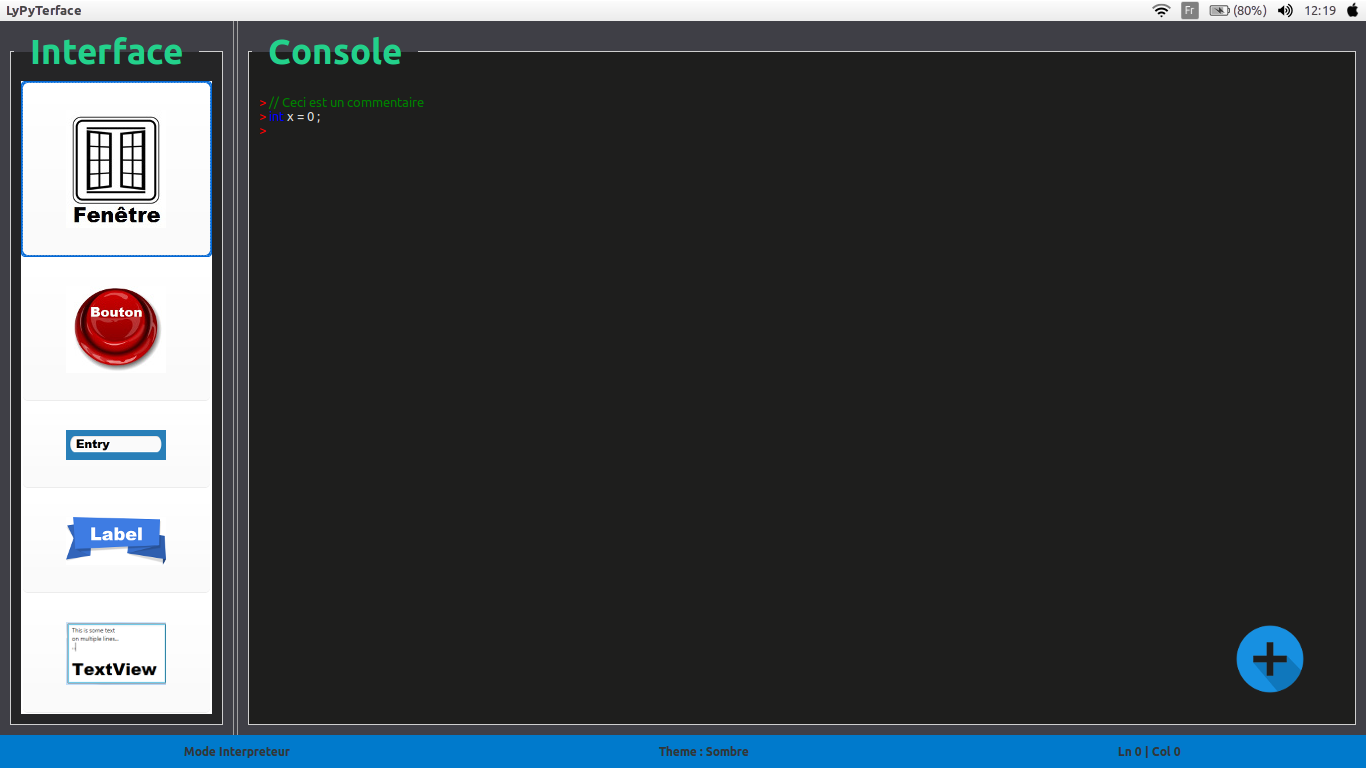
\includegraphics[width=0.75\textwidth]{IDE_1.png} 
   \caption{\label{étiquette} IDE de ShankSscript}
\end{figure}


\textbf{Remarque :} Cette plateforme et utilisé à la fois dans les systèmes Unix et Windows . 


\section{Premiers pas avec l'interpréteur de commandes ShankScript}

Après les premières notions théoriques et l'installation de ShankScript, il est temps de découvrir un peu l'interpréteur de commandes de ce langage. Même si ces petits tests vous semblent anodins, vous découvrirez dans ce chapitre les premiers rudiments de la syntaxe du langage et je vous conseille fortement de me suivre pas à pas, surtout si vous êtes face à votre premier langage de programmation.
\\[0.5cm]
Comme tout langage de programmation, ShankScript a une syntaxe claire : on ne peut pas lui envoyer n'importe quelle information dans n'importe quel ordre. Nous allons voir ici ce que ShankScript mange… et ce qu'il ne mange pas.

\subsection{L'interpréteur}

Eh bien, cet interpréteur de commandes va nous permettre de tester directement du code. Je saisis une ligne d'instructions, j'appuie sur la touche Entrée de mon clavier, je regarde ce que me répond ShankScript (s'il me dit quelque chose), puis j'en saisis une deuxième, une troisième… Cet interpréteur est particulièrement utile pour comprendre les bases de ShankScript et réaliser nos premiers petits programmes. Le principal inconvénient, c'est que le code que vous saisissez n'est pas sauvegardé (sauf si vous l'enregistrez manuellement, mais chaque chose en son temps).
\\[0.5cm]
Dans la fenêtre que vous avez sous les yeux, l'information qui ne change pas d'un système d'exploitation à l'autre est la série de trois chevrons qui se trouve en bas à gauche des informations : >. Ces trois signes signifient : « je suis prêt à recevoir tes instructions ».
\\[0.5cm]
Comme je l'ai dit, les langages de programmation respectent une syntaxe claire. Vous ne pouvez pas espérer que l'ordinateur comprenne si, dans cette fenêtre, vous commencez par lui demander : « j'aimerais que tu me codes un jeu vidéo génial ». Et autant que vous le sachiez tout de suite (bien qu'à mon avis, vous vous en doutiez), on est très loin d'obtenir des résultats aussi spectaculaires à notre niveau.
\\[0.5cm]
Tout cela pour dire que, si vous saisissez n'importe quoi dans cette fenêtre, la probabilité est grande que ShankScript vous indique, clairement et fermement, qu'il n'a rien compris.
\\[0.4cm]
Si, par exemple, vous saisissez « Salut ShankScript », vous allez avoir un message d'erreur qui dit que vous avez une erreur de syntaxe .
\\[0.5cm]
l'interpréteur vous indique qu'il a trouvé un problème dans votre ligne d'instruction. Il vous indique le numéro de la ligne (en l'occurence la première), qu'il vous répète obligeamment (ceci est très utile quand on travaille sur un programme de plusieurs centaines de lignes).  	 	


\subsection{Première commande}
On va commencer par la saisie des nombre et opération arithmétique ,Nous allons donc essayer d'obtenir les résultats de calculs plus ou moins compliqués:

\subsubsection{Saisir un nombre } 

Vous avez pu voir sur notre premier (et à ce jour notre dernier) test que ShankScript n'aimait pas particulièrement les suites de lettres qu'il ne comprend pas. Par contre, l'interpréteur adore les nombres. D'ailleurs, il les accepte sans sourciller, sans une seule erreur .
\\ Si vous entrer un nombre dans l'interpréteur ,alors sans problème il va l'afficher . ce simple retour indique que l'interpréteur a bien compris et que votre saisie est en accord avec sa syntaxe. De même, vous pouvez saisir des nombres à virgule.
\\[0.5cm]
\textbf{Remarque :} on utilise ici la notation anglo-saxonne, c'est-à-dire que le point remplace la virgule. La virgule a un tout autre sens pour ShankScript, prenez donc cette habitude dès maintenant.
\\[0.5cm]
Il va de soi que l'on peut tout aussi bien saisir des nombres négatifs (vous pouvez d'ailleurs faire l'essai).

\subsubsection{Opérations courantes} 

Les opérations disponibles en ce moment sont :Addition, soustraction, multiplication, division .
\\[0.5cm]
Pour effectuer ces opérations, on utilise respectivement les symboles +, -, * et /. 
\\[0.5cm]
On a aussi ajouté l'opération Modulo qui permet de connaître le reste de la division.


\section{Les variables}

\subsection{C'est quoi une variable ?}

Une variable est une donnée de votre programme, stockée dans votre ordinateur. C'est un code alpha-numérique que vous allez lier à une donnée de votre programme, afin de pouvoir l'utiliser à plusieurs reprises et faire des calculs un peu plus intéressants avec. C'est bien joli de savoir faire des opérations mais, si on ne peut pas stocker le résultat quelque part, cela devient très vite ennuyeux.
\\[0.5cm]
Voyez la mémoire de votre ordinateur comme une grosse armoire avec plein de tiroirs. Chaque tiroir peut contenir une donnée ; certaines de ces données seront des variables de votre programme.

\subsection{Comment cela fonctionne-t-il ?}
Le plus simplement du monde. Vous allez dire à Python : « je veux que, dans une variable que je nomme age, tu stockes mon âge, pour que je puisse le retenir (si j'ai la mémoire très courte), l'augmenter (à mon anniversaire) et l'afficher si besoin est ».
\\[0.5cm]
Comme on vous l'a dit, on ne peut pas passer à côté des variables. Vous ne voyez peut-être pas encore tout l'intérêt de stocker des informations de votre programme et pourtant, si vous ne stockez rien, vous ne pouvez pratiquement rien faire.
\\[0.5cm]
En ShankScript, pour donner une valeur à une variable, il suffit d'écrire nom de la  variable egal valeur.
\\[0.5cm]
Une variable doit respecter quelques règles de syntaxe incontournables :
\\[0.5cm]
\begin{enumerate}
\item Le nom de la variable ne peut être composé que de lettres, majuscules ou minuscules, de chiffres et du symbole souligné  (appelé underscore en anglais).
\item Le nom de la variable ne peut pas commencer par un chiffre.
\item Le langage Python est sensible à la casse, ce qui signifie que des lettres majuscules et minuscules ne constituent pas la même variable (la variable AGE est différente de aGe, elle-même différente de age).
\end{enumerate}

Au-delà de ces règles de syntaxe incontournables, il existe des conventions définies par les programmeurs eux-mêmes. L'une d'elles, que j'ai tendance à utiliser assez souvent, consiste à écrire la variable en minuscules et à remplacer les espaces éventuels par un espace souligné.
\\[0.5cm]
Et d'après de ce qu 'on a vu avant ,vous pouvez les même opérations arithmétiques sur les variables .
\\[1cm]
\textbf{Remarque :} Certains mots-clés de ShanskScript sont réservés, c'est-à-dire que vous ne pouvez pas créer des variables portant ce nom. Comme ("var","str","return","class","function" ...).


\subsection{Les types de données en ShankScript}
Là se trouve un concept très important, que l'on retrouve dans beaucoup de langages de programmation.
\\
\subsection*{Qu'entend-on par « type de donnée » ?}

Jusqu'ici, vous n'avez travaillé qu'avec des nombres. Et, s'il faut bien avouer qu'on ne fera que très rarement un programme sans aucun nombre, c'est loin d'être la seule donnée que l'on peut utiliser en ShankScript. À terme, vous serez même capables de créer vos propres types de données, mais n'anticipons pas.
\\[0.5cm]
ShankScript a besoin de connaître quels types de données sont utilisés pour savoir quelles opérations il peut effectuer avec. Dans ce chapitre, vous allez apprendre à travailler avec des chaînes de caractères, et multiplier une chaîne de caractères ne se fait pas du tout comme la multiplication d'un nombre. Pour certains types de données, la multiplication n'a d'ailleurs aucun sens. Python associe donc à chaque donnée un type, qui va définir les opérations autorisées sur cette donnée en particulier.
\subsection*{Les différents types de données}
\subsubsection*{Type entier et flottante}
Si on voit les langage de tels que C ,et va remarquer que chaque type est mis à part ,cela et bien mais notre but est de  rendre la programmation facile , on veut que l'utilisateur ne se soucie de rien qu'on il va commencer à programmer .
\\[0.5cm]
Alors on a rassemblé les deux types en un seul type qui est « var » , il peut contenir soit un flottant soit un entier par rapport à la situation .
\subsubsection*{Les chaînes de caractère }
Heureusement, les types de données disponibles en ShnkScript ne sont pas limités aux seuls nombres, bien loin de là. Le dernier type « simple » que nous verrons dans ce chapitre est la chaîne de caractères. Ce type de donnée permet de stocker une série de lettres, pourquoi pas une phrase.
\\[0.5cm]
On peut écrire une chaîne de caractères de cette façon :
\\
\textit{	entre guillemets ("ceci est une chaîne de caractères") .}



\section{Les structures conditionnelles}

Jusqu'à présent, nous avons testé des instructions d'une façon linéaire : l'interpréteur exécutait au fur et à mesure le code que vous saisissiez dans la console. Mais nos programmes seraient bien pauvres si nous ne pouvions, de temps à autre, demander à exécuter certaines instructions dans un cas, et d'autres instructions dans un autre cas.
\\[0.5cm]
Dans ce chapitre, on va vous parler des structures conditionnelles, qui vont vous permettre de faire des tests et d'aller plus loin dans la programmation.
\\[0.5cm]
Les conditions permettent d'exécuter une ou plusieurs instructions dans un cas, d'autres instructions dans un autre cas.
\\[0.5cm]
\subsection{La condition simple IF}

En anglais, le mot « si » se traduit parif. C'est celui qu'on utilise en langage C pour introduire une condition.
\\[0.5cm]
Écrivez donc unif. Ouvrez ensuite des parenthèses : à l'intérieur de ces parenthèses vous devrez écrire votre condition.
\\[0.5cm]
Ensuite, ouvrez une accolade{et fermez-la un peu plus loin}. Tout ce qui se trouve à l'intérieur des accolades sera exécuté uniquement si la condition est vérifiée.
\subsection{Le ElSE pour dire sinon}
Maintenant que nous savons faire un test simple, allons un peu plus loin : si le test n'a pas marché (il est faux), on va dire à l'ordinateur d'exécuter d'autres instructions.
\\[0.5cm]
Il suffit de rajouter le motelseaprès l'accolade fermante du if.
\\[0.5cm]
ALors si on applique la logique si l'action n'est pas inclus dans la condition <if> on swap directement à ELSE .


\subsection{LE ELSE IF pour dire sinon si}
On a vu comment faire un « si » et un « sinon ». Il est possible aussi de faire un « sinon si » pour faire un autre test si le premier test n'a pas marché. Le « sinon si » se place entre leifet leelse.
\\[0.5cm]
L'ordinateur fait les tests dans l'ordre.
\begin{enumerate}
\item D'abord il teste le premierif: si la condition est vraie, alors il exécute ce qui se trouve entre les premières accolades.
\item Sinon, il va au « sinon si » et fait à nouveau un test : si ce test est vrai, alors il exécute les instructions correspondantes entre accolades.
\item Enfin, si aucun des tests précédents n'a marché, il exécute les instructions du « sinon ».
\end{enumerate}
\textbf{Remarque :}Leelseet leelse ifne sont pas obligatoires. Pour faire une condition, seul unifest nécessaire (logique me direz-vous, sinon il n'y a pas de condition !).
\\[0.5cm]



\subsection{La condition Switch}
La conditionif... elseque l'on vient de voir est le type de condition le plus souvent utilisé.
En fait, il n'y a pas 36 façons de faire une condition en C. Leif... elsepermet de gérer tous les cas.
\\[0.5cm]
Les informaticiens détestent faire des choses répétitives, on a eu l'occasion de le vérifier plus tôt.
\\[0.5cm]
Alors, pour éviter d'avoir à faire des répétitions comme ça quand on teste la valeur d'une seule et même variable, ils ont inventé une autre structure que leif... else. Cette structure particulière s'appelle switch.
\\[0.5cm]
L'idée c'est donc d'écrireswitch (maVariable)pour dire « je vais tester la valeur de la variablemaVariable». Vous ouvrez ensuite des accolades que vous refermez tout en bas.
\\[0.5cm]
Ensuite, à l'intérieur de ces accolades, vous gérez tous les cas :case 2,case 4,case 5,case 45…
\\[0.5cm]
\textbf{Remarque :}Vous devez mettre une instructionbreak;obligatoirement à la fin de chaque cas. Si vous ne le faites pas, alors l'ordinateur ira lire les instructions en dessous censées être réservées aux autres cas ! L'instructionbreak;commande en fait à l'ordinateur de « sortir » des accolades.
\\[0.5cm]
Enfin, le casdefaultcorrespond en fait auelsequ'on connaît bien maintenant. Si la variable ne vaut aucune des valeurs précédentes, l'ordinateur ira lire ledefault.










\section{Les boucles}




\subsection{Qu'est-ce qu'une boucle ?}
une boucle est une structure qui permet de répéter les mêmes instructions plusieurs fois.
\\[0.5cm]
Tout comme pour les conditions, il y a plusieurs façons de réaliser des boucles. Au bout du compte, cela revient à faire la même chose : répéter les mêmes instructions un certain nombre de fois.
\\[0.5cm]
Voici ce qu'il se passe dans l'ordre :

\begin{enumerate}
\item l'ordinateur lit les instructions de haut en bas (comme d'habitude) ;
\item puis, une fois arrivé à la fin de la boucle, il repart à la première instruction ;
\item il recommence alors à lire les instructions de haut en bas…
\item … et il repart au début de la boucle.
\end{enumerate}
Le problème dans ce système c'est que si on ne l'arrête pas, l'ordinateur est capable de répéter les instructions à l'infini ! Il n'est pas du genre à se plaindre, vous savez : il fait ce qu'on lui dit de faire… Il pourrait très bien se bloquer dans une boucle infinie, c'est d'ailleurs une des nombreuses craintes des programmeurs.
\\[0.5cm]
Et c'est là qu'on retrouve… les conditions ! Quand on crée une boucle, on indique toujours une condition. Cette condition signifiera « Répète la boucle tant que cette condition est vraie ».
[0.5cm]
Comme je vous l'ai dit, il y a plusieurs manières de s'y prendre. Voyons voir sans plus tarder comment on réalise une boucle de type while .


\subsection{La boucle while}
C'est aussi simple que cela. while signifie « Tant que ». On dit donc à l'ordinateur « Tant que la condition est vraie, répète les instructions entre accolades ».
\\[0.5cm]
L'ordinateur lit la condition ,après il teste si la condition est vrai ,si la condition est vrai il execute le programme et refais le teste,sinon il sort .
\\[0.5cm]
Lorsque vous créez une boucle, assurez-vous toujours qu'elle peut s'arrêter à un moment ! Si la condition est toujours vraie, votre programme ne s'arrêtera jamais !
\subsection{La boucle do… while}
Ce type de boucle est très similaire à while, bien qu'un peu moins utilisé en général.
La seule chose qui change en fait par rapport à while, c'est la position de la condition. Au lieu d'être au début de la boucle, la condition est à la fin .
\\[0.5cm]
Qu'est-ce que ça change ?
\\[0.5cm]
Pour la boucle do… while, c'est différent : cette boucle s'exécutera toujours au moins une fois. En 
\\[0.5cm]
Il est donc parfois utile de faire des boucles de ce type, pour s'assurer que l'on rentre au moins une fois dans la boucle.
\\[0.5cm]
\textbf{Remarque :}Il y a une particularité dans la boucle do… while qu'on a tendance à oublier quand on débute : il y a un point-virgule tout à la fin ! N'oubliez pas d'en mettre un après le while, sinon votre programme plantera à la compilation !
\\[0.5cm]
\subsection{La boucle for}
En théorie, la boucle while permet de réaliser toutes les boucles que l'on veut.\\
Toutefois, tout comme le switch pour les conditions, il est dans certains cas utile d'avoir un autre système de boucle plus « condensé », plus rapide à écrire.
\\[0.5cm]
Les boucles for sont très très utilisées en programmation. Je n'ai pas de statistiques sous la main, mais sachez que vous utiliserez certainement autant de for que de while, si ce n'est plus, il vous faudra donc savoir manipuler ces deux types de boucles.
\\[0.5cm]
Comme je vous le disais, les boucles for sont juste une autre façon de faire une boucle while.
\\[0.5cm]

\section{Les entrées et les sorties}
(En cours ...)
\section{Les fonctions}
(En cours ...)
\section{Les packages}
(En cours ...)
\section{Interfaçage et les packages graphiques}
(En cours ...)